% !TEX root =  thesis.tex
\chapter{Detailed System Description}\label{detailedSystemDescription}

\section{Design overview}

The system is broken into five major packages called application, input, output, simulation, and tasktree. Figure 5.1 shows the relationship between these components.

\begin{figure}[htb]
\centering
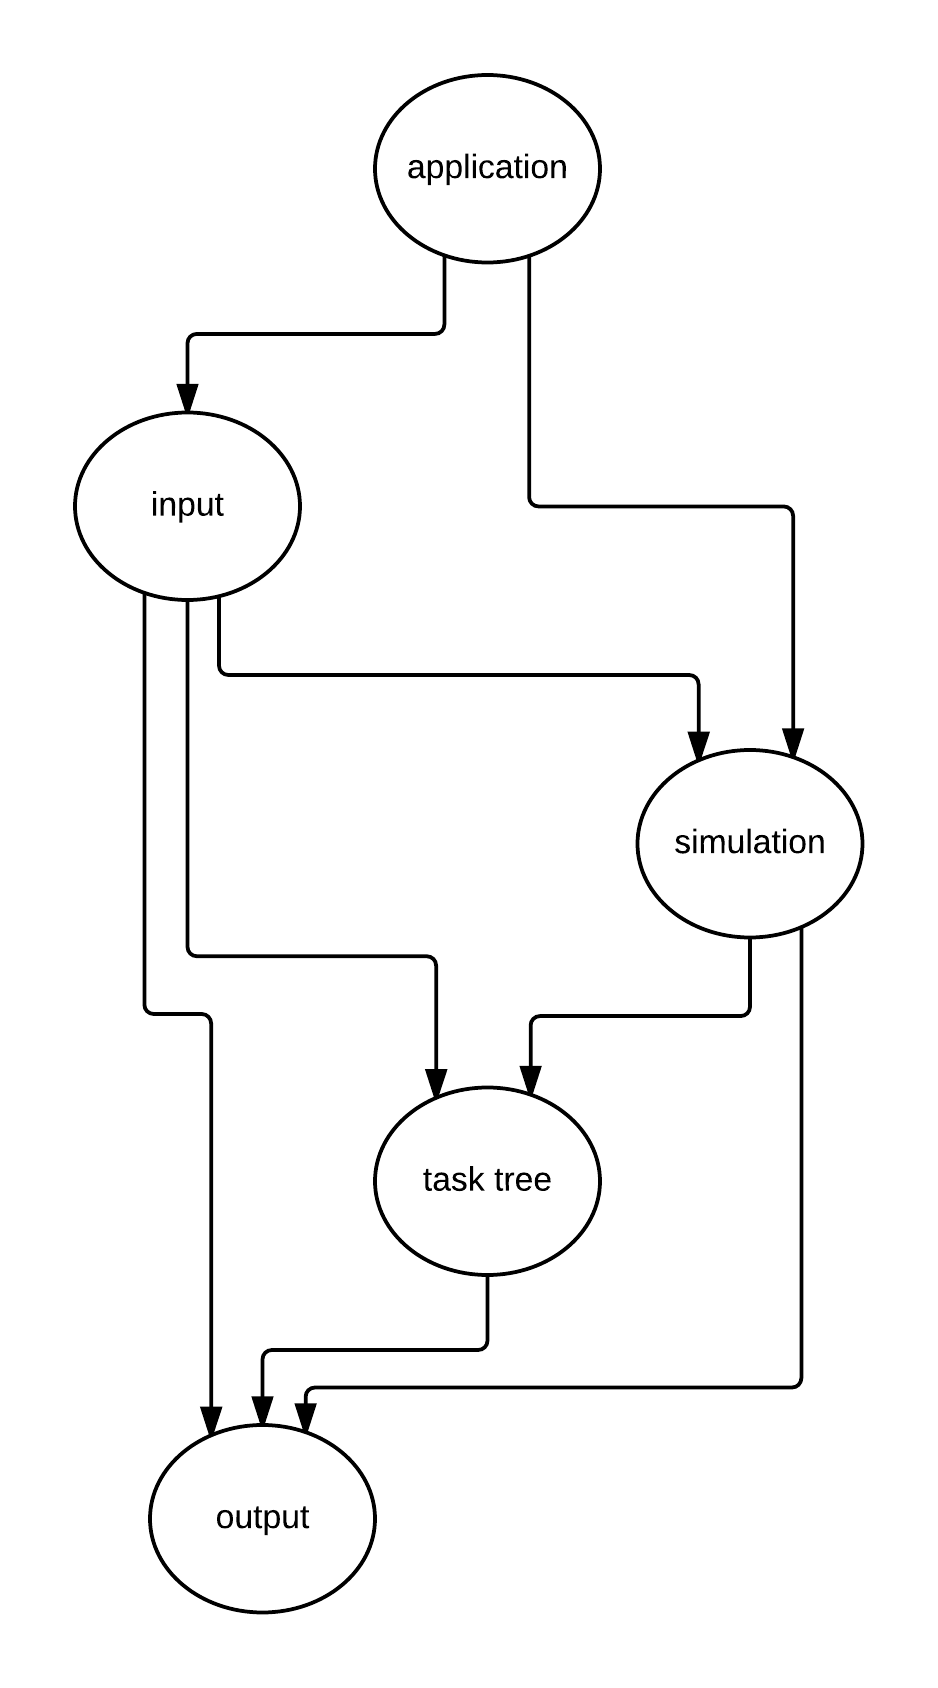
\includegraphics[width=2.0in]{figs/UsesDiagram}
\caption{Uses diagram for packages within MASS.}
\label{fig:UsesDiagram }
\end{figure}

\section{Package Overview}

\begin{enumerate}

\item\textbf{application}
\begin{itemize}
\item Description: The application package is responsible for initializing the other packages. 
\item Contains: The application package contains module AISim.
\item Uses: The application package does not use any other packages.
\end{itemize}

\item\textbf{input}
\begin{itemize}
\item Description: The input package is responsible for reading the initial data input and building a Task Tree to represent this data.
\item Contains: The input package contains three modules which include Parser, ConfigurationData, and InputData.
\item Uses: This package uses the tasktree package.
\end{itemize}

\item\textbf{output}
\begin{itemize}
\item Description: The Output Package is responsible for logging data after the simulation has completed.
\item Contains: The output package contains a module Logger.
\item Uses: This package uses the simulation package
\end{itemize}

\item\textbf{simulation}
\begin{itemize}
\item Description : The simulation package is responsible for connecting and communicating with agents, managing the tasktree, and advancing the clock.
\item Contains : This package contains the modules Simulator, Agent, EventManager, Message and Thread.
\item Uses : This package uses the input Package.
\end{itemize}

\item\textbf{tasktree}
\begin{itemize}
\item Description : The tasktree package is responsible for representing the Task Tree in a hierarchical manner that is easy for the simulation package to update and distribute. Figure 5.2 represents the Uses diagram for the package tasktree.
\item Contains : This package contains the modules Node, NodeRelationship, and Distribution.
\item Uses : This package uses the output package.

\begin{figure}[htb]
\centering
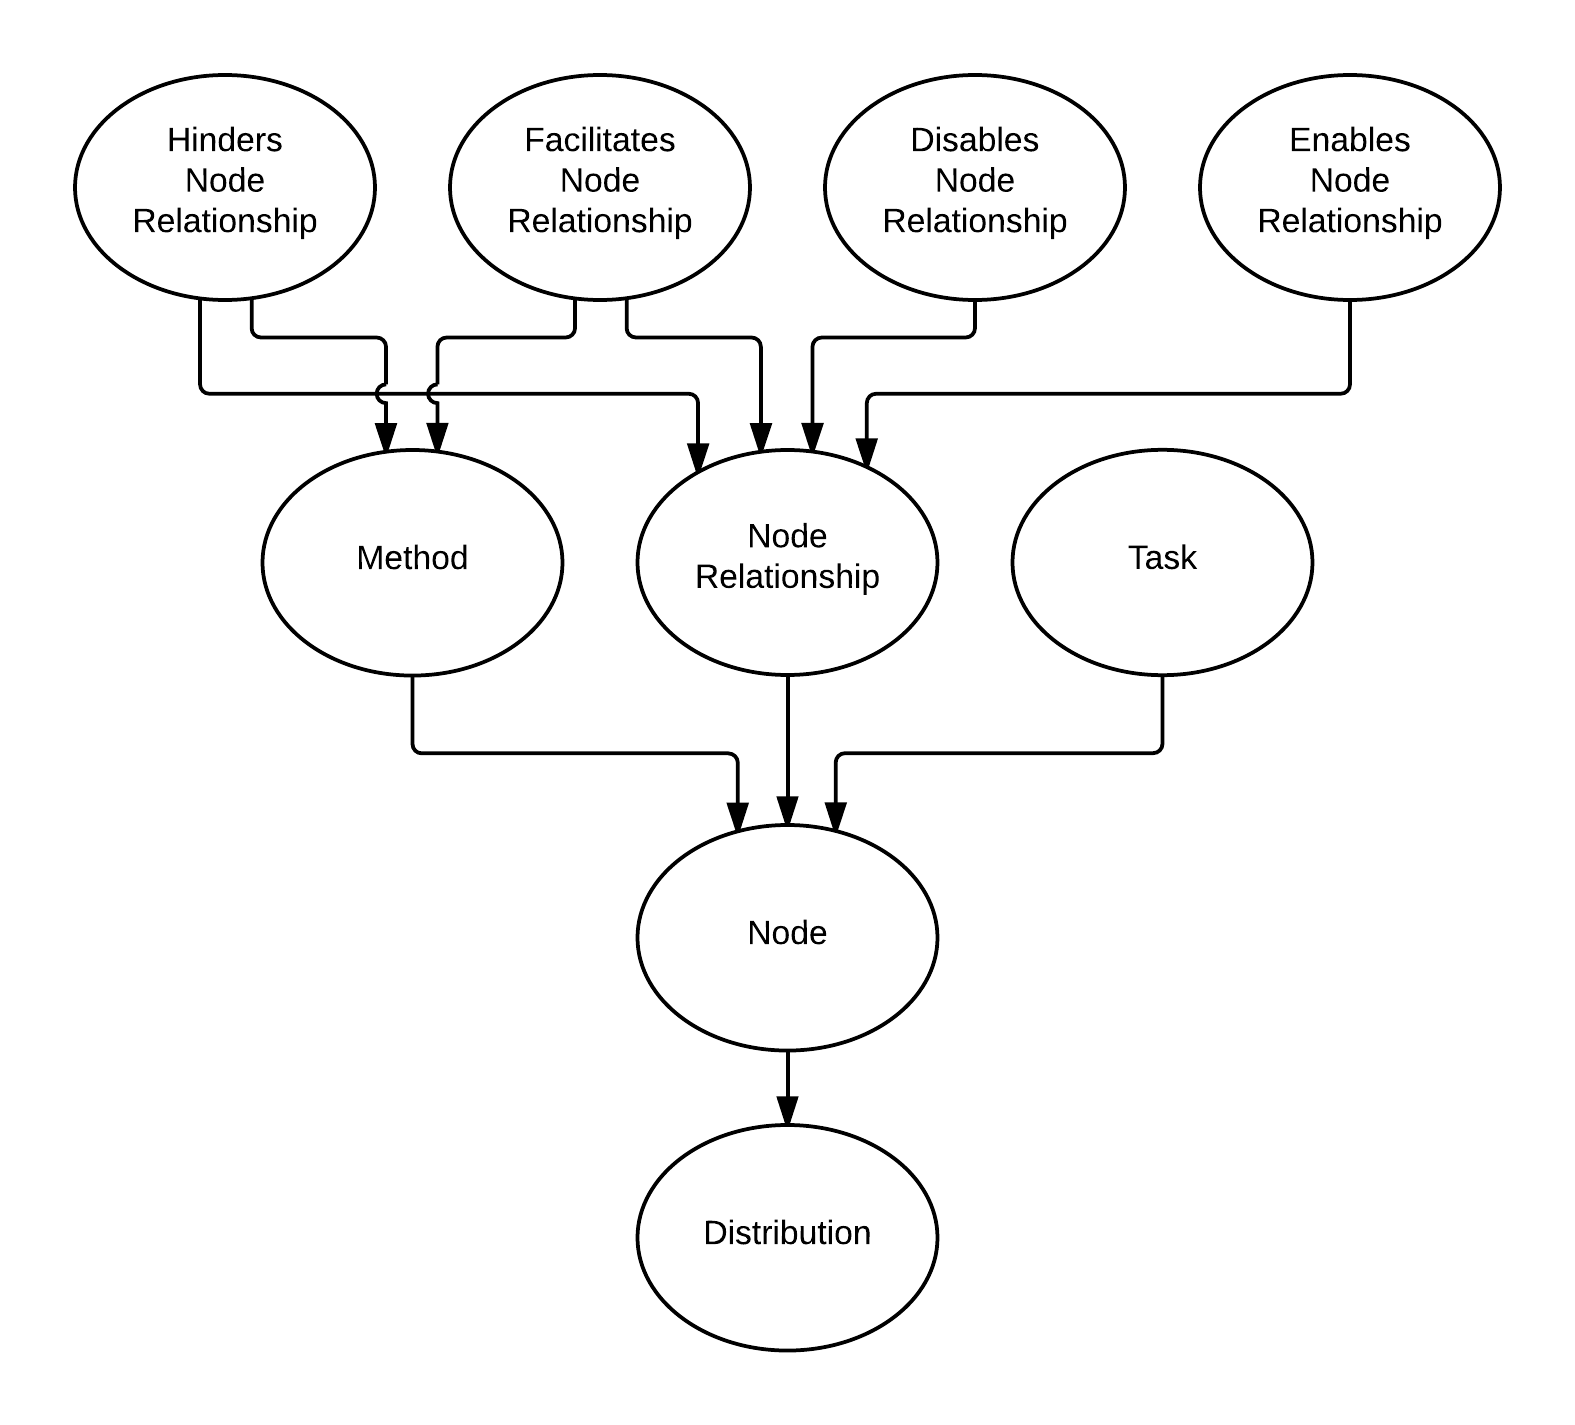
\includegraphics[width=4.5in]{figs/tasktree}
\caption{Uses diagram for the package tasktree}
\label{fig:tasktree}
\end{figure}


\end{itemize}

\end{enumerate}

\section{Detailed Package Design}

\begin{enumerate}

\item \textbf{Application}  The application package is responsible for initializing the modules within the input and simulation packages in order to begin the Simulation.

\begin{figure}[htb]
\centering
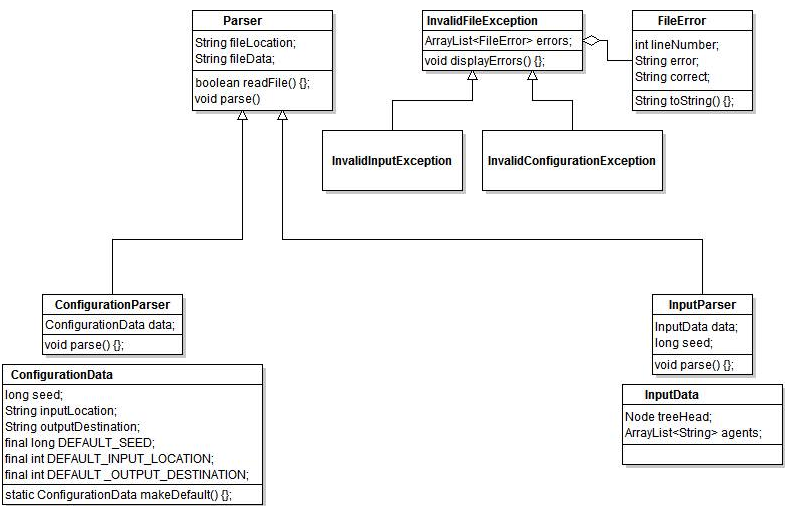
\includegraphics[width=5.0in]{figs/input}
\caption{UML diagram for input package}
\label{fig:input}
\end{figure}

\item \textbf{Input} Figure 5.3 represents the UML diagram for input package. This package is responsible for reading and parsing the cTAEMS SFI and the plain text CFI. This packages contains an abstract parser which serves as a template for the InputParser and the ConfigurationParser. \\

\begin{itemize}
\item \textbf{InputParser}: The InputParser is responsible for reading the SFI which contains definitions for Agents, Events and relationships that make up the Simulation. The first step of the parse involves reading the desired cTAEMS file into a string by implementing Java's BufferedReader class. Second, the string is split into tokens such as Agent, Task, TaskGroup, and Method. These tokens are further parsed in order to analyze their various components. For example, a Task could be broken up into a label, list of Subtasks and a function of Quality which are instantiated into the corresponding data structure. This data will be stored in the InputData class which will then be passed to the simulation. \\

\item \textbf{ConfigurationParser}: The configuration parser reads and parses the CFI to determine the random seed used throughout the Simulation. The Configuration parser will use Java's BufferedReader class to read in the file, with the first line representing the seed, the second the input location and lastly the output destination. This data is written to the ConfigurationData class which is sent to the simulator. \\

\item \textbf{Exceptions}: Within the input package there are three exceptions which are used to report a problem encountered during a parse. These exceptions are: InvalidFileException, InvalidInputException, and InvalidConfigurationException. \\
\end{itemize}

\begin{figure}[htb]
\centering
\includegraphics[width=2.0in]{figs/output}
\caption{UML diagram for output package}
\label{fig:output}
\end{figure}

\item \textbf{Output} Figure 5.4 represents the UML diagram for output package. The output package is responsible for logging data after the simulation has completed. It contains a Logger class which upon completion will create the LFO document. \\

\begin{itemize}
\item \textbf{Logger}: The Logger class is responsible for producing a  transcript of Agent communication, statistics on Agent communication frequency, and the intermediate and final Quality, Cost, and Duration that results from completing an Event in the Task Tree. Data will be passed to the Logger by the modules within the simulation package as the simulation advances. Upon completion of a simulation, the Logger will compile statistics on agent communication and produce the LFO containing the previously mentioned data. \\
\end{itemize}
\begin{figure}[htb]
\centering
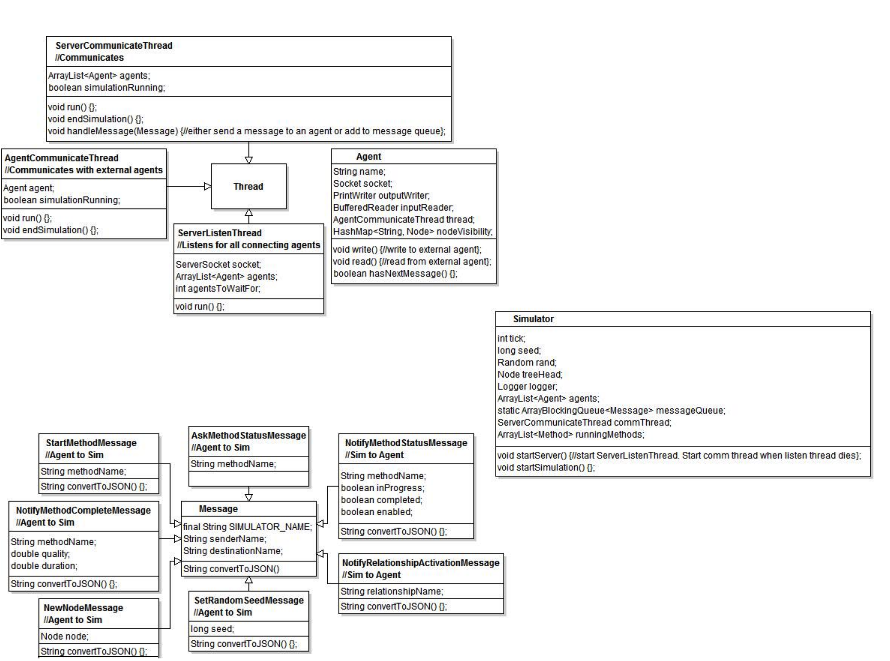
\includegraphics[width=6.0in]{figs/Simulation}
\caption{UML diagram for Simulation package}
\label{fig:Simulation}
\end{figure}

\item \textbf{Simulation}  Figure 5.5 represents the UML diagram for simulation package. The simulation package is responsible for handling all of the communications with Agents as well as updating the tasktree architecture to model the current state of the simulation. \\

\begin{itemize}
\item \textbf{Simulator}: This class contains all of the information about the simulation such as the random number seed, the head Node of the tasktree, the list of currently connected Agents, the Logger object, the incoming Message queue, the list of currently running Methods, and the ServerCommunicateThread. This class is the core timekeeper of the simulation. \\

\item \textbf{Agent}: This class is used to encapsulate all the relevant information about an Agent such as its name, Socket, and HashMap of visible Nodes. This class also contains a PrintWriter, BufferedReader, and AgentCommunicateThread used to communicate with the Agent program that it represents. \\

\item \textbf{ServerListenThread}: This Thread will listen for new Agents that are trying to connect to the simulation. If an Agent connects at the correct time and with the correct name then this thread packages the Agent's information into an Agent object so that it can be accessed and communicated with throughout the simulation. \\

\item \textbf{ServerCommunicateThread}: This Thread will create and process all Messages comming in from and going out to all Agents in the simulation. \\

\item \textbf{AgentCommunicateThread}: This Thread will send and recieve Messages to and from a given Agent. \\

\item \textbf{Message}: This class contains the base information for a Message such as the name of the Simulator, the senderName, and the destinationName. There are many subtypes of Messages listed below. \\

\subitem \textbf{(i) StartMethodMessage}: Tells the Simulator that the Agent wants to start a Method.
\subitem \textbf{(ii) AskMethodStatusMessage}: Ask the Simulator for the status of a currently running Method.
\subitem \textbf{(iii) NotifyMethodStatusMessage}: Tells an Agent the status of a currently running Method.
\subitem \textbf{(iv) NotifyMethodCompleteMessage}: Tells an Agent that their Method has completed and what the result is.
\subitem \textbf{(v) NewNodeMessage}: An Agent tells the Simulator to add a Node to the tasktree.
\subitem \textbf{(vi) SetRandomSeedMessage}: Tells an Agent to set their random number seed to a specified number.
\subitem \textbf{(vii) NotifyRelationshipActivationMessage}: Tells an Agent that a NodeRelationship was activated and what the result is. \\
\end{itemize}

\begin{figure}[htb]
\centering
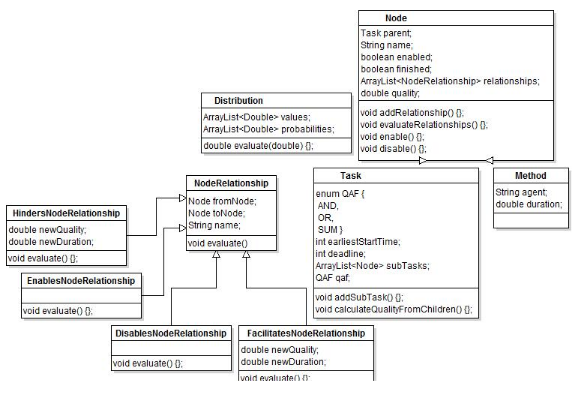
\includegraphics[width=6.0in]{figs/TaskTreeUML}
\caption{UML diagram for tasktree package}
\label{fig:TaskTreeUML}
\end{figure}

\item \textbf{Tasktree} This package provides a framework for building a Task Tree. It is used by the input package to construct a programmatic representation of the SFI including Task, Methods, and Node relations. \\

\begin{itemize}
\item \textbf{Node}: The base node class that contains all the information about a Node of the tasktree such as Quality, name, this Nodes parent Node, a list of NodeRelationships from this Node, whether or not the Node is enabled, and whether or not the Node is finished. \\

\item \textbf{Task}: A Task is a type of node whose completion is defined by its Subtasks. A Task's completion quality is the result of its subtasks. Either the Sum of the Quality of the Subtasks, the highest Quality of any Subtask, or the lowest Quality of any Subtask. More Quality options can be added as needed. A Subtask can either be another Task which would have more Subtasks or a Method which has no Subtasks. \\

\item \textbf{Method}: A Method is a node that can be completed by an Agent. The Method contains a Duration which is the amount of time it takes to complete the Method. Methods can have their Duration and Quality modified by the FacilitatesNodeRelation and HindersNodeRelation. \\

\item \textbf{NodeRelations}: There are many NodeRelations that represent the affect that the completion of one Node has on another. The types of NodeRelations are below. \\

\subitem \textbf{(i) HindersNodeRelation}: Completing one Node decreases the Quality and increases the Duration of another Node.

\subitem \textbf{(ii) FacilitatesNodeRelation}: ompleting one Node increases the Quality and decreases the Duration of another Node.

\subitem \textbf{(iii) EnablesNodeRelation}: The completion of the first Node enables the completion of the second Node

\subitem \textbf{(iv) DisablesNodeRelation}: The completion of the first Node disables the completion of the second Node.

\item \textbf{Distribution}  A distribution is used to generate Qualities and Durations for the Nodes.


\end{itemize}
\end{enumerate}